%& -aux-directory=/tmp
% sorgt  dafuer dass aux files sonstwohin kommen -output-directory=C:/pdfout
\documentclass[10pt,a4paper, fleqn]{article}
% twocol class oder so geht auch
% fleqn macht align formeln nach lings
\usepackage[utf8]{inputenc}
\usepackage{hyperref}
\hypersetup{linktocpage}
%\usepackage[ngerman]{babel}
\usepackage[american]{babel}
\usepackage{amsmath} % xrightarrow, ...
\usepackage{cite}
\usepackage{units} % nicefrac
\usepackage{datetime} % fuer Uhrzeit im \date
%\usepackage{wrapfig} % bilder rechts
\usepackage{caption} % fuer subcaption
\usepackage{subcaption} % subfigures
\usepackage{graphicx} % Bilder allgemein einbinden
%\usepackage{tabularx} % Tabellen
\usepackage{lastpage} % Anzahl Seiten
\usepackage{multicol} % zweispaltige Titelseite
\usepackage{a4wide} % bessere Papiernutzung
\usepackage{fancyhdr} % Header/Footer
%\pagestyle{fancy} % Kopf/Fussbereich der Seiten
\usepackage{amssymb} % therefore = dreieckdots
\usepackage{array} % tables
\usepackage{booktabs} % better tables
\usepackage{floatrow} % caption beside image
\usepackage[toc,page]{appendix}
\usepackage{mathtools} % ceil, floor
\DeclarePairedDelimiter\ceil{\lceil}{\rceil}
\DeclarePairedDelimiter\floor{\lfloor}{\rfloor}

\usepackage[usenames,dvipsnames]{color} % more colors

% zweispaltiger Text
\usepackage{multicol}
%\setlength{\columnseprule}{0.4pt}

% Ueberschriften kleiner 	
%\usepackage{titlesec}
%\titleformat{\section}{\large\bfseries}{\thesection}{1em}{}
%\titlespacing{\paragraph}{%
%  0pt}{%              left margin
%  0.5\baselineskip}{% space before (vertical)
%  1em}%               space after (horizontal)
%%\titlespacing{\section}{0pt}{0.2\baselineskip}{0.1\baselineskip}
%\titlespacing{\align}{0pt}{0.2\baselineskip}{0.1\baselineskip}
%\titlespacing{\equation}{0pt}{0.2\baselineskip}{0.1\baselineskip}

% abgefahrenes highlighting von formeln
\usepackage{xcolor}
% klappt net, was einfacheres:
\newcommand{\highlight}[1]{%
  \colorbox{green!30}{$\displaystyle#1$}}
  
% Hübsche Boxen
% Alternative dazu (gut fuer Seitenanmerkungen):
% http://tex.stackexchange.com/a/73418/49958
% \usepackage[draft]{todonotes}   % notes showed
\usepackage{mdframed}
\mdfdefinestyle{todo}{
	linecolor=red,
	backgroundcolor=yellow!40,
	linewidth=5pt,
	topline=false,
	rightline=false,
	bottomline=false
}
% definiere \begin{todo} und \todo{blabla} auf einmal:
\usepackage{environ}
\NewEnviron{todo}%[1]
  {\begin{mdframed}[style=todo]
  	 \BODY
   \end{mdframed}\vspace{.3cm}}

% Kopfzeile/Fusszeile mit fancy
%\fancyhead{}
%\fancyfoot{}
%\fancyfoot[FL]{\slshape F-Praktikum, Supraleiter}
%\fancyfoot[FR]{\slshape Page \thepage {} / \pageref*{LastPage}}
%\renewcommand{\headrulewidth}{0 pt}

% Bibliography
\bibliographystyle{ieeetr}

% Farben (werden derzeit nur in hypersetup verwendet)
\usepackage{color}
\definecolor{darkblue}{rgb}{0,0,.6}
\definecolor{darkred}{rgb}{.1,0,0}
\definecolor{darkgreen}{rgb}{0,.5,0}

% Schriften
% Palatino for rm and math | Helvetica for ss | Courier for tt
\usepackage{mathpazo} % math & rm
\linespread{1.05}        % Palatino needs more leading (space between lines)
\usepackage[scaled]{helvet} % ss
\usepackage{courier} % tt
\normalfont
\usepackage[T1]{fontenc}

% Hyperref aufsetzen
\hypersetup{
    pdftitle={Master Physik bei Nicolini, Calc writeup},
    pdfauthor={Sven Köppel},
    pdfsubject={master},
    pdfkeywords={physik} {master} {uni} {frankfurt} {fias},
    colorlinks=true,        % test: stat gerahmten Links
    linkcolor=red,          % color of internal links
    citecolor=darkgreen,    % color of links to bibliography
    filecolor=darkred,      % color of file links
    urlcolor=cyan           % color of external links
}

% Allgemeine Meta-Daten, derzeit ungenutzt
\title{\vspace{-9ex} Calc14 \vspace{-1ex}} % vertikalen platz weg...
\author{\small %
\href{https://itp.uni-frankfurt.de/~koeppel}{Sven Köppel} \\
\small \texttt{koeppel@fias.uni-frankfurt.de}}
\date{\small Generation date: \today, \currenttime}


\begin{document}
\maketitle

% abkuerzungen:
\renewcommand{\d}{\mathrm{d}}
\newcommand{\dd}[2]{\frac{\mathrm{d} #1}{\mathrm{d} #2}}
\newcommand{\pp}[2]{\frac{\partial #1}{\partial #2}}
\renewcommand{\L}{L_P}
\newcommand{\pr}{p_r}
\newcommand{\psenk}{p_\perp}
\newcommand{\ebenso}{\biggl( ~ \therefore ~ \biggr) }
\newcommand{\metrik}[1]{\d s^2 = \left( #1 \right) \d t^2 \left( #1 \right)^{-1} \d r^2 + r^2 \d \Omega_{D-2}^2 }
\newcommand{\winkel}{r^2 \d \Omega^2}
\newcommand{\dann}{$\rightarrow~$}
\newcommand{\CA}{ {\cal A}}
\newcommand{\C}[1]{ {\cal #1}}
\newcommand{\mn}{_{\mu\nu}}

% colored symbols:
% http://tex.stackexchange.com/questions/85033/colored-symbols
\newcommand*{\mathcolor}{}
\def\mathcolor#1#{\mathcoloraux{#1}}
\newcommand*{\mathcoloraux}[3]{%
  \protect\leavevmode
  \begingroup
    \color#1{#2}#3%
  \endgroup
}
% In Text: $a\textcolor{red}{\ast}b$
% In Math: $a\mathcolor{red}{\ast}b$
\newcommand{\redmin}{\mathcolor{red}{-}}
\newcommand{\redplus}{\mathcolor{red}{+}}
\newcommand{\pn}{\mathcolor{OliveGreen}{+ n}}
\newcommand{\n}{ {\mathcolor{OliveGreen}{n}} }

\begin{multicols}{2}
\begin{abstract}
In this document, I consider an alternative non vanishing
$[x_i, p_j] = \Theta_{ij}$ for GUP in $n$ spatial
extra dimensions. I will show the connection to my previous
holographic and self-encoding calculations with the
Heaviside step function $\Theta \ to H$ smearing.

We will see, that in order to give self-regular solutions, the
GUP function $f(\beta \vec p)$ must scale with the number of
extra dimensions. Otherwise, integral divergences cannot be
cured.

This work closes up with  the Knipfer2014 paper (in progress).
\end{abstract}
\vfill
\columnbreak
\tableofcontents
\end{multicols}

\section{GUP in Large Extra Dimensions}
In the Isi 2013 paper, the GUP
\begin{equation}
[x^i, p_j] = i \delta^i_j (1 + \beta \vec p^2)
\end{equation}
was explored. Isi and Knipfer currently work on exploiting this equations in $n$ total spatial dimensions, by using the identity
\begin{equation}
1 = \int_{-\infty}^{+\infty} \frac{\d^n p}{1 + \beta \vec p^2} \mid p \rangle \langle p \mid
\label{eq:identity}
\end{equation}
proposed by Kempf1995. It feels like this smearing is not »strong enough« for fighting against nominator $p$ powers, as Nicolini outlined:
\begin{equation}
\int \frac{p^{n-1} \d^n p}{1 + \beta \vec p^2}
\sim
\int p^ {n-3} \d p
\end{equation}
An appealing approach is switching to another GUP. Indeed, Kempf showed that for the general case, \eqref{eq:kempf1} and \eqref{eq:kempf2} can be proposed. Nicolini deduced \eqref{eq:kempf3} at the 03.Jun Group meeting (yet possibly without proof):
\begin{subequations}
\begin{align}
\label{eq:kempf1}
[x_i, p_j] &= i\hbar\delta_{ij} \left(1 + f(\vec p^2) \right) \\
\label{eq:kempf2}
[x_i, x_j] &= -2 i \hbar f'(\vec p^2) \left( x_i p_j - x_j p_i \right) \\
\label{eq:kempf3}
1 &= \int \frac{\d^n p}{1 + f(\vec p^2)}
\end{align}
\end{subequations}

The important question of the freedom of arbitrary choice of $f(\vec p^2)$ arises. It is this if \eqref{eq:identity} depends on the eikonal approximation made by Amati, Ciafaloni, Vereziano at string scattering computations (...).

Simpleminded, I will ignore this question and perform a calculation with $f(\vec p^2) = L_p^{n-1} p^{n-1}$, where $p=\sqrt{\vec p^2}$.

\subsection{$H$-model theory}
\begin{todo}
Diesen Abschnitt hab ich nur eingefügt, um einen Zusammenhang zu
meinen bisherigen Untersuchungen zu beschreiben. Mir ist aufgefallen,
dass der gar nicht so wirklich vorhanden ist. Die Integrale sind
allenfalls ähnlich, aber das GUP-Zeug kann man nur {\it unbequem}
als $H(r)$-Funktion benutzen. Der Begriff {\it $H$-model theory}
ist für diesen Zusammenschrieb frei erfunden.
\end{todo}

The last 6 months, I was busy exploiting the mathematical properties of modified Schwarzschild-Blackholes in higher dimensions. The modification always entered by smearing the Heaviside Theta distribution $\Theta(r) \to H(r)$. Thereby,
\begin{equation}
\rho(r) = \frac{M}{\Omega_{2+n} r^{2+n}} \delta(r) \to \frac{M}{\Omega_{2+n} r^{2+n}} \dd{H(r)}{r}
\end{equation}
with $\Omega_d$ the surface of an $d$-sphere (see e.g. Calc11 for a complete summary of my formalism). Note that $H(r)$ is a placehoder for a concrete function profile typically denoted by a lowercase letter like $h(r)$.

Lately I was supposed to bring my holographic and self-encoding approaches, which were modeled in 4d with models,
\begin{itemize}
\item Holographic: $H(r) = h(r) := r^2 / (r^2 + L^2)$,
\item Self-Encoding: $H(r) = h_\alpha(r) := r^3 / (r^\alpha + L^\alpha /2)^{3/\alpha}$,
\item Bardeen: $H(r) = h_e(r)$, a special choice of $\alpha$ in $h_\alpha$,
\end{itemize}
to a more fundamental principle: By finding a bilocal smearing operator $\C A^2(x-y)=\C A^2(\square)$ which acts on the Ricci scalar, one finds the modified Einstein Equations which contain delta-smearing according to the model choice of $H(r)\in \{ h, h_\alpha, h_b, \dots \}$.

I found that one can connect that $H$-model framework with the determination of $\CA^2$ by the expression
\begin{equation}
\C A^{-2}(p^2) = \frac{1}{\Omega_{n+2}} \int \d^{3+n} z~ \underbrace{\frac 1{z^{2+n}} \dd{H}{z}}_{:= V(z)} e^{-i \vec p \cdot \vec z}
\end{equation}
I usually solved this $3+n$-dimensional Fourier Transformation by integrating out $n+1$ angels, which yields an effective one-dimensional Fourier integral with an assembled, artificially looking Fourier kernel. I worked on these expressions for one month. See Calc12 and Calc13 for the detailed derivation.
\begin{subequations}
\begin{align}
\mathcal{I} = \int \d^{3+n} \vec z ~ V(|z|) e^{-i \vec p \vec z}
= \frac{1}{2 \Omega_{n+2}}
\frac{2\pi i}p \int_{-\infty}^{\infty} \d z ~v(z) e^{-ipz}
\end{align}
with the Fourier kernel
\begin{equation}
v(z) = z^{1+n} \left( V(z)\Theta(z) + (-1)^n V(-z)\Theta(-z) \right)
\end{equation}
In $H$-formalism, $V(z) := z^{-(2+n)} \dd{H}{z}$ and therefore
\begin{equation}
v(z) = z^{1+n} \left( \frac{1}{z^{n+2}} \dd Hz \Theta(z) + \frac{(-1)^n}{(-z)^{n+2}} \dd Hz (-z) \Theta(-z) \right)
\end{equation}
\end{subequations}
As told in Calc13, by construction $v(z)$ is always odd and therefore $\C I$ always Real in any number of dimensions.

\section{GUP: The Mass}
The $\CA^{-2}$-smearing in the Knipfer2014 paper was performed like
\begin{equation}
\CA^{-2}(\square) \delta(\vec x) \propto
\int \frac{e^{i\vec x \vec p}}{1 + \beta p^2} \d^3 p
\label{eq:bigV}
\end{equation}
%
Despite the fact that the integration direction is virtually inversed, I think this can be clearly identified to my calculations, defacto working with the integration kernel
%
\begin{equation}
p^{1+n} \dd{h(p)}{p} = \frac 1{1+\beta p^2} = V(p)
\end{equation}

\subsection{GUP as $H$-model theory?}
As it is described in the next sections, the integrals look really very similar to the Holographic Metric integrals. I wonder if there is any deeper connection.

\subsection{Switching to $3+n$ dimensions in dimensionless coordinates}
We now modify \eqref{eq:bigV} in two ways: Tuning up the powers of $p$ and absorbing $\sqrt{\beta}=L_p$ in the dimensionless variable $q$:
\begin{equation}
V(p) = \frac{1}{1+L_p^{n+2} p^{n+2}} = \frac 1{1 + q^{n+2}}
\label{eq:Vn}
\end{equation}
The coordinate shift $q=pL$ is also done in the integration measure: $\d p = \d q / L$. So I am about to solve the integral
\begin{subequations}
\begin{align}
\label{eq:I1}
\C I &=
\underbrace{\frac{1}{(2\pi)^{3+n}}}_{\text{inv Four suppr.}}
 \frac{2\pi i}r \int_{-\infty}^\infty
\d p~
p^{1+n}
\left(
\frac{1}{1 + q^{n+2}} \Theta(q)
+ (-1)^n
\frac{1}{1 + (-q)^{n+2}} \Theta(-q)
\right)
~e^{ipr} \\
&=  \frac{2\pi i }{zL} \int_{-\infty}^\infty
\d p~
\frac{q^{1+n}}{L^{1+n}}
\left(
\frac{1}{1 + q^{n+2}} \Theta(q)
+ (-1)^n
\frac{1}{1 + (-q)^{n+2}} \Theta(-q)
\right)
~e^{ipz}
\label{eq:I2}
\end{align}
\end{subequations}
where the dimensionless $z=r/L$ is determined by requiring $e^{ipr} = e^{iqz}$. From \eqref{eq:I1} to \eqref{eq:I2} we note that the dimensionless calculation requires a global $\frac 1{L^{2+n}}$ scaling.

\subsection{The poles}
Consider the poles of \eqref{eq:Vn}. They are given by
\begin{equation}
1 + q^{n+2} = 0
\quad\Leftrightarrow\quad
q = (-1)^{\frac 1{n+2}}
=\exp\left\{
\frac{i\pi + 2\pi i k}{n+2}
\right\}
\quad
\forall k\in \mathbb{N_0}
\end{equation}
There are $n+1$ poles (different choices for $k$), given by $k=0,1,\dots,n,n+1$.

As far as I see, these poles are absolutely equal to the Holographic poles. So perhaps see Calc11 for a nice plot of these poles in $n\in[0,7]$ dimensions.

\subsection{Performing Cauchy theorem} \label{heading:cauchy1}
In Calc13, the Cauchy theorem steps are explained in detail. I won't retrace them here. Actually, for $n=0$ the integral can be easily made by hand because there is only one pole to consider. One archieves
\begin{equation}
\C I = \frac{2\pi e^z}{L^2 z} = \frac{2\pi e^{r/L}}{L r}
= \frac{2 \pi e^{r/\sqrt{\beta}} }{\sqrt\beta r}
\end{equation}
This is the same as in equation (7) in Knipfer2014.

The expressions for higher $n$ get really long. I have not yet found short summation or recursion relations. I think the most outstanding
problem is that the expressions are purely $\in \mathbb{C} \setminus \mathbb{R}$, c.f. table \ref{table:A}.

The further calculation of $\C M(R)$ can be in principle made (I actually think one even can express that in terms of $\gamma(s,x)$ functions), but they inherit the complex value.

\begin{table}
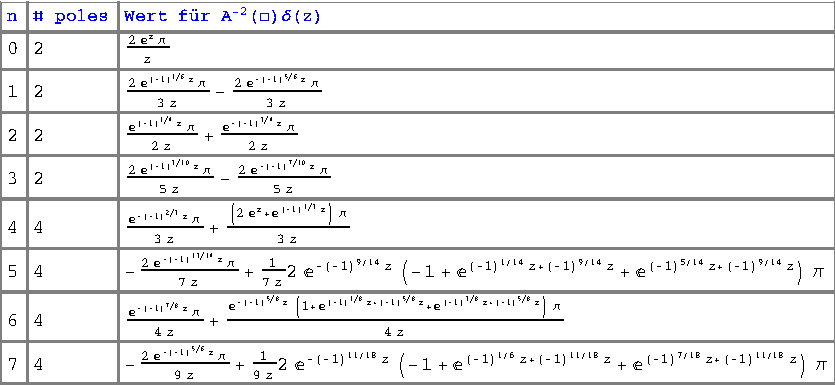
\includegraphics[width=\textwidth]{plots/A-table.pdf}
\caption{Values for $\C A^{-2}$ as derived in section \ref{heading:cauchy1} for different number of extra dimensions $n$.}
\label{table:A}
\end{table}



\end{document}
